\let\negmedspace\undefined
\let\negthickspace\undefined
\documentclass[journal]{IEEEtran}
\usepackage[a5paper, margin=10mm, onecolumn]{geometry}
\usepackage{lmodern} % Ensure lmodern is loaded for pdflatex
\usepackage{tfrupee} % Include tfrupee package

\setlength{\headheight}{1cm} % Set the height of the header box
\setlength{\headsep}{0mm}     % Set the distance between the header box and the top of the text

\usepackage{gvv-book}
\usepackage{gvv}
\usepackage{cite}
\usepackage{amsmath,amssymb,amsfonts,amsthm}
\usepackage{algorithmic}
\usepackage{graphicx}
\usepackage{textcomp}
\usepackage{xcolor}
\usepackage{txfonts}
\usepackage{listings}
\usepackage{enumitem}
\usepackage{mathtools}
\usepackage{gensymb}
\usepackage{comment}
\usepackage[breaklinks=true]{hyperref}
\usepackage{tkz-euclide} 
\usepackage{listings}
\usepackage{gvv}                                        
\def\inputGnumericTable{}                                 
\usepackage[latin1]{inputenc}                                
\usepackage{color}                                            
\usepackage{array}                                            
\usepackage{longtable}                                       
\usepackage{calc}                                             
\usepackage{multirow}                                         
\usepackage{hhline}                                           
\usepackage{ifthen}                                           
\usepackage{lscape}
\begin{document}

\bibliographystyle{IEEEtran}
\vspace{3cm}

\title{7-7.2-20}
\author{EE24BTECH11005 - Arjun Pavanje}
% \maketitle
% \newpage
% \bigskip
{\let\newpage\relax\maketitle}
Question:\\
Find the area of the region bounded by the curve $y^2=4x, x^2=4y$
\begin{table}[h!]    
  \centering
  \begin{tabular}[12pt]{ |c| c|}
    \hline
    \textbf{Variable} & \textbf{Description}\\ 
    \hline
	$\vec{a}$ & $BC$ line\\
   \hline
	$\vec{b}$ & $AC$ line\\
   \hline
	$\vec{c}$ & $AB$ line, $5cm$ length\\
   \hline
	$\vec{K}$ & $a+b=5cm$\\
	\hline
	$\vec{\angle{A}}$ & $\angle{BAC}=45{\degree}$\\
	\hline

    \end{tabular}

  \caption{Variables Used}
  \label{tab1-1.9-6}
\end{table}\\
\solution
The general equation of a parabola with directrix $\vec{n}^{\top}\vec{x}=c$ is given by,
\begin{align}
	g\brak{\vec{x}}=\vec{x}^{\top}\vec{V}\vec{x}+2\vec{u}^{\top}\vec{x}+f=0\\
	\vec{V}=\norm{\vec{n}}^2\vec{I}-e^2\vec{n}\vec{n}^{\top}\\
	\vec{u}=ce^2\vec{n}-\norm{\vec{n}}^2\vec{F}\\
	f=\norm{\vec{n}}^2\norm{\vec{F}}^2-c^2e^2
\end{align}
for the parabola $y^2=4x$, equation of directrix is, $\myvec{-1&0}\vec{x}=1$
\begin{align}
	\vec{V}&=\myvec{0&0\\0&1}\\
	\vec{u}&=\myvec{-2\\0}\\
	f&=0
\end{align}
for the parabola $x^2=4y$, equation of directrix is, $\myvec{0&-1}\vec{x}=1$
\begin{align}
	\vec{V}&=\myvec{1&0\\0&0}\\
	\vec{u}&=\myvec{0\\-2}\\
	f&=0
\end{align}
The intersection of two conics with parameters $\vec{V}_i,\vec{u}_i,f_i, i=1,2$ is defined as,
\begin{align}
	\vec{x}^{\top}\brak{\vec{V}_1-\vec{V}_2}\vec{x}+2\brak{\vec{u}_1-\vec{u_2}}^{\top}\vec{x}+\brak{f_1-f_2}=0
\end{align} 
On solving we get the points of intersection to be $\myvec{0\\0},\myvec{4\\4}$
Area between the 2 parabolas is,
\begin{align}
	&\int_0^4 2\sqrt{x}dx- \int_0^4 \frac{x^2}{4}dx = \frac{16}{3}
\end{align}
The area between the curves $y^2=4x, x^2=4y$ is, $\frac{16}{3}$ units
\begin{figure}[h!]
   \centering
   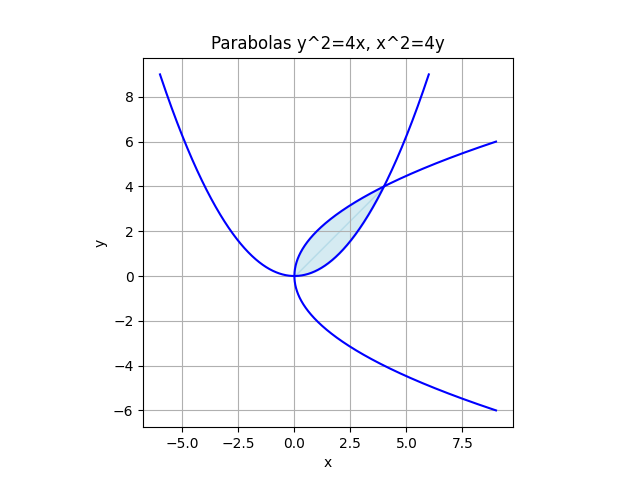
\includegraphics[width = 1\linewidth]{figs/fig.png}
   \caption{Required Parabolas}
   \label{stemplot}
\end{figure}
\end{document}
